\documentclass{article}

% PACKAGES =====================================================
% font settings
\usepackage{titlesec}
\usepackage{lmodern}
\usepackage[T1]{fontenc} % For improved sans-serif font
% Change title format to sans-serif
\titleformat{\title}{\sffamily\LARGE\bfseries}{}{0pt}{}
% Change section format to sans-serif
\titleformat{\section}{\sffamily\Large\bfseries}{}{0pt}{}
% Change subsection format to sans-serif
\titleformat{\subsection}{\sffamily\large\bfseries}{}{0pt}{}
% Change subsubsection format to sans-serif
\titleformat{\subsubsection}{\sffamily\normalsize\bfseries}{}{0pt}{}
% page settings
\usepackage[a4paper,scale=0.8]{geometry}
% language settings
\usepackage[american]{babel}
% captions settings
\usepackage{caption}
\captionsetup{labelfont={small,sf,bf}}
\setlength\belowcaptionskip{5pt}
% graphics settings
\usepackage{graphicx}
% tweaking the footnotes
\usepackage[hang,flushmargin]{footmisc}
% bibliogrpahy
\usepackage[backend = biber, autolang=other, style = nature]{biblatex}
\addbibresource{my_bib.bib}
% graph creation
\usepackage{tikz}
\usepackage{float}
% hyperref
\usepackage{hyperref}
% table settings
\usepackage{multirow}
\usepackage{csvsimple}
% float barrier
\usepackage{placeins}
% list settings
\usepackage{enumitem}
% figure settings
\usepackage{subcaption}

% code settings
\usepackage{listings}
\usepackage{xcolor}

\lstdefinestyle{mystyle}{
  backgroundcolor=\color{white},   % choose the background color
  basicstyle=\ttfamily\footnotesize, % size of fonts used for the code
  keywordstyle=\color{blue},	     % color of keywords
  commentstyle=\color{green!60!black}, % color of comments
  stringstyle=\color{red},	     % color of strings
  numberstyle=\tiny\color{gray},   % style of line numbers
  breaklines=true,		     % automatic line breaking
  captionpos=b, 	     % position of the caption
  frame=single, 	     % adds a frame around the code
  numbers=left, 	     % where to put the line numbers
  numbersep=5pt,		     % how far the line numbers are from the code
  showspaces=false,		     % show spaces adding particular underscores
  showstringspaces=false,	     % underline spaces within strings
  showtabs=false,		     % show tabs within strings adding particular underscores
  tabsize=2			     % sets default tabsize to 2 spaces
}
\lstset{style=mystyle}

% header settings
\usepackage{fancyhdr}
\pagestyle{fancy}
\fancyhf{} % Clear all header and footer fields
\fancyfoot[C]{\thepage} % Add page numbering to the center footer

\renewcommand{\headrulewidth}{0pt} % Remove horizontal line from header
% first page customization
\fancypagestyle{plain}{
  \fancyhead[L]{\textit{Lisa PARUIT}- Internship Report 2A}
  % Left header
  \fancyhead[R]{
    \raisebox{-0.4\height}{\includegraphics[height=1.2cm]{Images/APTlogosignature.jpg}}
    \raisebox{-0.3\height}{\includegraphics[height=1cm]{Images/logo_universidad_barcelona_nuevo.jpg}}
  }}

% title settings
\title{\sffamily\LARGE\bfseries Internship report 2A}
\author{\sffamily Research assistant at the University of Barcelona
  \\Lisa PARUIT}
\date{}

% BEGIN DOC ====================================================
\begin{document}
\maketitle

% title of abstract in english
\renewenvironment{abstract}
{\begin{center}\textbf{Summary}\end{center}}{}

\begin{abstract}
  \noindent \textbf{Introduction} I was hired as a research assistant in the
  agroecology department of the University of Barcelona. This was an unpaid
  insternship in which I was given the opportunity to work on a meta-analysis
  of
  LCA studies of cocoa and chocolate bars prodcuction.\\
  \textbf{Methods} In facts, I almost lead the project on my own, from the
  database design to the data extraction, analysis and interpretation. As I
  didn't get much guidance, I took a few false directions that however allowed
  me
  to draw on knowledge and skills I have acquired throughout my studies in
  AgroParisTech and face the challenges of a researcher's work.\\
  \textbf{Results} Since most of my time was spent in paper reading and I had
  to adopt a trial and error approach, which is very time consuming, I didn't
  have time to gather enough data to get significant results. This report
  however
  details the methodology used for analysis and the material I created for this
  purpose.\\
  \textbf{Conclusion} Although I was disappointed that my internship wasn't as
  instructive in terms of scientific content and methods than I had expected due
  to
  lack of guidance, it conforted me in the path of scientific research and was 
  a great mean
  to experience the day-to-day life of a researcher. I also had fun being on my
  own and having to adopt a genuine sientific method to conduct my project.
\end{abstract}

% second abstract in french
\renewenvironment{abstract}
{\begin{center}\textbf{Résumé}\end{center}}{}

\begin{abstract}
  \noindent \textbf{Introduction} J'ai été prise comme assistante de recherche
  au sein du département d'agroécologie de l'Université de Barcelone. Il
  s'agissait d'un stage non rémunéré au cours duquel j'ai eu l'occasion de
  travailler sur une méta-analyse des études d'Analyse de Cycle de Vie de la
  production de cacao et de barres chocolatées.\\
  \textbf{Méthodologie} Dans les faits, j'ai presque dirigé le projet moi-même,
  de la conception de la base de données à l'interprétation des résultats, en
  passant par l'analyse des données et le développements d'outils informatiques
  pour les exploiter. Comme j'ai été peu encadrée, j'ai parfois suivi des
  pistes
  erronées qui m'ont toutefois permises de tirer profit des connaissances et
  des
  compétences que j'ai acquises au cours de mes études à AgroParisTech et de me
  confronter aux défis quotidiens du travail de chercheur.\\
  \textbf{Résultats} Comme j'ai passé la plupart de mon temps sur la
  bibliographie et que j'ai été contrainte d'adopter une approche par essais et
  erreurs très chronophage, je n'ai pas eu le temps de rassembler suffisamment
  de données pour obtenir des résultats satisfaisants.
  La méthodologie utilisée pour l'analyse et les outils que j'ai créé à cette
  fin sont cependant détaillés dans ce rapport.\\
  \textbf{Conclusion} J'ai été déçue que mon stage n'ait pas été
  aussi instructif que je l'attendais en termes de contenu et de méthodes
  scientifiques en
  raison d'un manque d'encadrement. Cette expérience m'a cependant confortée
  dans la voie de la recherche et a été un
  excellent moyen de m'essayer au quotidien du chercheur. J'ai également trouvé
  une forme de satisfaction dans le fait d'être livrée à moi-même face à un
  problème donné et de devoir adopter une véritable démarche scientifique pour
  mener à bien ce projet.
\end{abstract}

\vspace{2cm}

\noindent \textit{\textbf{À l'intention de l'examinateur:} Ce document a été 
implémenté avec LaTeX. La police par défaut étant Times New Roman 10pt au lieu
des 12pt recommandés par l'école, le nombre de page s'en trouve par conséquent
réduit par rapport à l'ampleur du contenu. L'utilisation de LaTeX a été motivée
par (i) la pertinence de maîtriser ce langage dans le monde de la recherche (ii)
la facilité de mise en page permise par le logiciel. D'autre part, ce rapport a
été rédigé en anglais pour des raisons de cohérence avec le stage que j'ai
effectué et des différentes notes méthodologiques que j'ai pu réaliser pour 
l'équipe.}

% TABLE OF CONTENTS =====================================================
\newpage
\tableofcontents
\newpage

% =======================================================================

% INTRODUCTION =====================================================
\section{Introduction} \label{sec:intro}
\subsection{Description of the institution and personal motivation}
The University of Barcelona (UB) is a public university located in Barcelona,
Spain
and the national leader in terms of research \cite{UBwebsite1}. Interested in
agronomical research with a specific focus on how to apply knowledge and
methods in ecology to the development of more resilient production systems, I
was attracted to this university as it hosts a research department focusing
solely on agroecology. Moreover, Spain being a major farming country in Europe,
I was eager to learn more about the challenges in this sector and how
agroecology research was lead there to tackle them.\\
I was very interested in the project currently lead by the department, focusing
on biodiversity restauration and understanding its involvement in agricultural
systems \cite{UBwebsite2}. I therefore contacted Dr. Xavier Sans Serra who was
already very busy but kindly redirected me to Laura Armengot Martinez, newly
arrived to the lab and who was already working on several projects.

\subsection{Job description and content}
After a time in the private sector, Dr. Armengot Martinez joined the UB's
agroecology lab back, where she did her pHD and her first steps in research.
Her focus was mainly on cocoa production and agricultural practices comparison
with an emphasis on agroforestery.\\
During our first meeting, Laura had told me she expected data from an
experimental station in Ecuador where trials on the performance of
aggroforestery in cocoa production were conducted. Unfortunately, the data was not yet
available yet when I arrived to the lab and we had to find another project to work
on. I was therefore redirected on a meta-analysis project focusing on the
environmental impact of cocoa and chocolate bar production.\\
\subsubsection{Mission content}
The project goal was to conduct a meta-analysis of the environmental impact of cocoa
and chocolate production as a tool for companies to assess their impact and
improve their practices. Laura and the paper co-leader had already selected
about 40 papers to base the analysis on. I was therefore assigned to
litterature review and data extraction from these papers. The data was to be
stored in a database and analyzed to provide a comprehensive and accessible
overview of chocolate production impact based on Life Cycle Analysis method.\\

% CONTEXT =====================================================
\section{Context of the study: impact studies in the food industry}
\input{SEC1 Scientific context}

% MATERIALS AND METHODS ========================================
\section{Material \& methods: database design}
\subsection{First project: creation of a comprehensive tool for data storage}
\subsubsection{Motivations}
This meta-analysis was first thought of to provide a comprehensive and
accessible overview of the environmental impact of chocolate production with a
emphasis on the distribution of this impact between different steps and actors
of the value chain. In the direction given by the paper's leaders, the results
were meant to adress to companies and eventually consumers. I therefore
suggested to create an app that would easily allow the user to:
\begin{enumerate}[label=\textbf{\roman*.}]
  \item Get a quick overview of the each step of the value chain's impact,
        with filtering tools and a graphic representation of the data.
  \item Compare the impact of different practices, countries, or value chains
        through a graphic representation of the required data.
  \item Access raw data and the references used to extract it, to allow for a
        more in-depth analysis and a review of the data.
  \item Eventually allow companies and actors to input their own data on the
        condition it is legitimately sourced.
\end{enumerate}

\subsubsection{Implementation with SQL and Python}
The app was to be built using SQL for the database manipulation and requests as
well as Python for the interactive program and the graphic interface. 
The database was built up as shown in \autoref{fig:database}.\\\\

\begin{figure}[htbp]
  \centering
  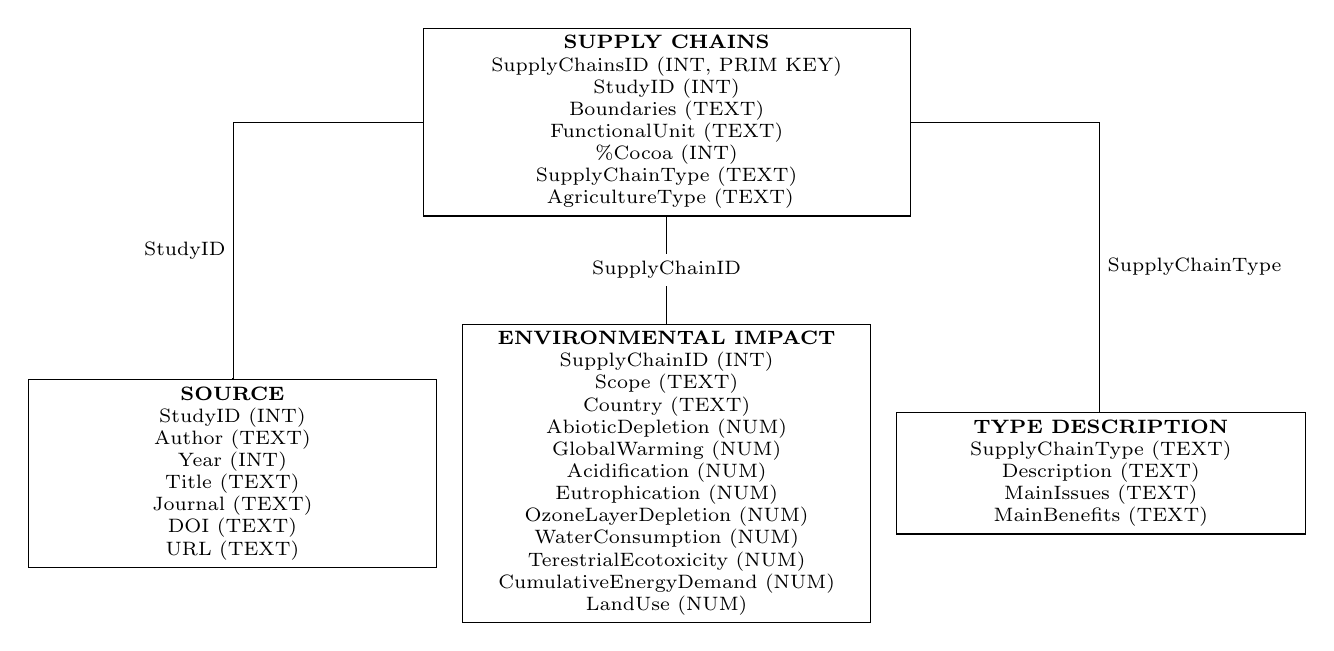
\begin{tikzpicture}[node distance=2cm]
    \scriptsize
    % Nodes
    \node (item1) [rectangle, draw, minimum width=2cm, minimum height=1cm]
    {\parbox{6 cm}{\centering \textbf{SUPPLY CHAINS}\\ SupplyChainsID (INT,
        PRIM
        KEY)\\ StudyID (INT) \\ Boundaries (TEXT) \\ FunctionalUnit (TEXT) \\
        \%Cocoa
        (INT) \\SupplyChainType (TEXT) \\ AgricultureType (TEXT) }};
    \node (item2) [rectangle, draw, minimum width=2cm, minimum height=1cm,
      below of=item1, yshift = -70] {\parbox{5cm}{\centering
        \textbf{ENVIRONMENTAL
          IMPACT} \\ SupplyChainID (INT) \\ Scope (TEXT) \\ Country (TEXT) \\
        AbioticDepletion (NUM) \\ GlobalWarming (NUM) \\ Acidification (NUM) \\
        Eutrophication (NUM) \\ OzoneLayerDepletion (NUM) \\ WaterConsumption
        (NUM) \\
        TerestrialEcotoxicity (NUM) \\ CumulativeEnergyDemand (NUM) \\ LandUse
        (NUM)
      }};
    \node (item3) [rectangle, draw, minimum width=2cm, minimum height=1cm, left
      of=item2, xshift = -100] {\parbox{5cm}{\centering \textbf{SOURCE} \\
        StudyID
        (INT) \\ Author (TEXT) \\ Year (INT) \\ Title (TEXT) \\ Journal (TEXT)
        \\ DOI
        (TEXT) \\ URL (TEXT) }};
    \node (item4) [rectangle, draw, minimum width=2cm, minimum height=1cm,
      right of=item2, xshift = 100] {\parbox{5cm}{\centering \textbf{TYPE
          DESCRIPTION} \\ SupplyChainType (TEXT) \\ Description (TEXT) \\
        MainIssues
        (TEXT) \\ MainBenefits (TEXT) }};

    % Links
    \draw [-] (item1) -- (item2) node[midway, fill = white]{SupplyChainID};
    \draw [-] (item1.west) -- ++(-2.4,0) |- (item3.north) node[near start,
        left]{StudyID};
    \draw [-] (item1.east) -- ++(2.4,0) |- (item4.north) node[near start,
        right]{SupplyChainType};
  \end{tikzpicture}
  \caption{Graph of the SQL database design. Tables are represented as squares
    while nodes represent the linking item between the database's tables.}
  \label{fig:database}
\end{figure}

\noindent The app was built up using tkinter and gave an interface as shown in
\autoref{fig:my_images}. Original files can be found on the Github page
associated to this project (cf.\autoref{sec:Access}). For now and since this
part of the project was given up upon, the app contains the following
functionality:
\begin{enumerate}[label=\textbf{\roman*.}]
  \item an interactive database structure graph to visualize and modify raw
        database
  \item a table display function from which data can be altered by
        doublclicking on item
  \item a path to add data to the database.
\end{enumerate}

\begin{figure}[htbp]
  \centering
  \begin{subfigure}[b]{0.4\textwidth}
    \includegraphics[width=\textwidth]{Images/Graph_interface_menu.png}
    \caption{Main page of the app prototype}
    \label{fig:my_image1}
  \end{subfigure}
  \hfill
  \begin{subfigure}[b]{0.58\textwidth}
    \includegraphics[width=\textwidth]{Images/graph_interface_table.png}
    \caption{Data display and modification window that appears when double
      clicking on an item.}
    \label{fig:my_image2}
  \end{subfigure}
  \caption{Image captures from the app prototype. On figure (a) is written
    \textit{ "Welcome to the database management app! This is an interactive
      map of
      the Chocolate \& Cocoa Value Chains Assessment Database. To view the data
      within
      a table, click on the name of the table. You will be able to edit the
      date from
      this new window. To enter new data from the literature, click on ADD DATA
      below."}}\label{fig:my_images}
\end{figure}

\subsubsection{Issues encountered and project redirection}
After some time, Laura and her collegue decided the app was not necessary. The
development of the code into an actual app would have required more
ressources to be allocated to the project and follow up with the UB's informatic
services. The app was therefore put on hold and it was decided the database
would be implemented using Excel.

\hspace{2cm}

\subsection{Final project : Excel database}
\subsubsection{Motivations}
Spreadsheet softwares are widely used tools in the industry as well as in
research labs and are accessible to most users. Laura and her collegue were not
familiar with SQL nor Python and were thus affraid not to be able to take over
the project when my internship would come to an end. Hence, it was decided to 
implement the database using Excel, although the goal of the app was to design
an ergonomic tool.

\subsubsection{Description of the database}
\input{SEC2 Description of the database}

% RESULTS =====================================================
\section{Preliminary results}
\input{SEC3 Results}

% DISCUSSION =====================================================
\section{Conclusion and personal insights}
\subsubsection{A disappointing turn of events...}
This internship was an opportunity for me to discover the world of research in
agroecology in a way that I was expecting to be thorough. The initial
project was to analyse data acquired over 10 years of experimental agroforestry
surveys. As I want to specialise more in statistical modelling and applied
mathematics, I see agroecology studies as statistical exploration of an
environment shaped by ecological interactions and natural hazards. The change
of project was therefore a great disappointment as I was expecting to focus on
data analysis and statistical modelling.

\subsubsection{...and a lack of guidance...}
I also found that my supervisor, like the rest of the researchers in the
department, seemed poorly organised and rather involved in their teaching
activities than in their research work. Laura, although reachable, was very
busy during my time in Barcelona and seemed unsure of what I could bring to the
table. I have the feeling that I have been put on a project out of spite rather
than necessity for the research team and that my added
value as an M1 engineering student was far from being fully used.
I would certainly have benefited more from this internship in terms of
knowledge deepening and new skills development if I had had more guidance on
this project.

\subsubsection{...which lead to a great learning experience!}
As I was instructed to start the project without any clear guidelines, I had to
be very proactive, suggest and support ideas that I was then able to test by
myself in a scientific approach. In a way, I had a free rein
on this project, which meant I faced a number of pitfalls that I
might have avoided if I had been better supervised. Although I would have
preferred to get more out of my time in the lab by being supported more, I
appreciated this freedom, which also allowed me to confront with no
concessions the day-to-day decision making and challenges of an actual
researcher.

\subsubsection{Conclusion}
I will take something very positive from this experience: I
love research and its conundrums. Although most of my time was spent
doing literature review and filling out the database, I very much enjoyed the
more creative moments that were also part of my work. The need to stand back,
zoom in and out during both the reflection and the realisation as well as the
need to think the project globally  were a pleasure and very instructive. I think
I managed to draw on the skills and knowledge I had acquired during my studies
whenever I could and to be critical in the light of this knowledge and the
objectives that were set.

\newpage
% APPENDICES =====================================================
\appendix

\section{A. Github repository} \label{sec:Access}

\subsection{General Github commit link:}
\url{https://github.com/lisaparuit/LCA-for-cocoa-and-chocolate-production-database}\\\\

\subsection{Other links:}
\textbf{Prototype app folder:}
\url{https://github.com/lisaparuit/LCA-for-cocoa-and-chocolate-production-database/blob/lisaparuit-prototype-app/New_app}\\
\textbf{Associated SQL database:}
\url{https://github.com/lisaparuit/LCA-for-cocoa-and-chocolate-production-database/blob/lisaparuit-prototype-app/ProjectUB.db}\\
\textbf{Final Excel database:}
\url{https://github.com/lisaparuit/LCA-for-cocoa-and-chocolate-production-database/blob/main/Chocolate%20LCA.xlsx}
\\\\All the other programms/files mentioned in this report can be found on the
general github link.

\section{B. Impossibility of sample size estimation}\label{sec:sample_sizing}
\input{APP1 sample_size_estimation}

\section{C. Code for results extraction and statistical
  analysis}\label{sec:stat_ana_code}
\input{APP2 code_for_stats_analysis}

% BIBLIOGRAPHY =====================================================
\printbibliography
\end{document}